% ═══════════════════════════════════════════════════════════════════════════
% IEEE Conference Paper — Alture AI
% A Hybrid Multi-Modal NLP Architecture for Explainable ATS Resume–Job 
% Compatibility and Reciprocal Recommendation
%
% Authors: Ahmad Mustafa Iqbal
% Department of Computer Science, COMSATS University Islamabad, Islamabad Campus
% ═══════════════════════════════════════════════════════════════════════════
\documentclass[conference]{IEEEtran}

% ── Packages ──
\usepackage{cite}
\usepackage{amsmath,amssymb,amsfonts}
\usepackage{algorithmic}
\usepackage{graphicx}
\usepackage{textcomp}
\usepackage{xcolor}
\usepackage{booktabs}
\usepackage{hyperref}
\usepackage{multirow}
\usepackage{url}
\usepackage{float}
\usepackage{microtype}

\hypersetup{
    colorlinks=true,
    linkcolor=black,
    citecolor=blue,
    urlcolor=blue,
}

\def\BibTeX{{\rm B\kern-.05em{\sc i\kern-.025em b}\kern-.08em
    T\kern-.1667em\lower.7ex\hbox{E}\kern-.125emX}}

\begin{document}

% ═══════════════════════════════════════════════════════════════════════════
% Title & Authors
% ═══════════════════════════════════════════════════════════════════════════
\title{Alture AI: A Hybrid Multi-Modal NLP Architecture for Explainable ATS Resume--Job Compatibility and Reciprocal Recommendation}

\author{
    \IEEEauthorblockN{Ahmad Mustafa Iqbal}
    \IEEEauthorblockA{
        \textit{Department of Computer Science} \\
        \textit{COMSATS University Islamabad, Islamabad Campus} \\
        Islamabad, Pakistan \\
        Email: ahmadmustafaiqbal@gmail.com
    }
}

\maketitle

% ═══════════════════════════════════════════════════════════════════════════
% Abstract
% ═══════════════════════════════════════════════════════════════════════════
\begin{abstract}
Applicant Tracking Systems (ATS) serve as the primary automated gatekeepers in modern corporate recruitment pipelines. However, conventional ATS algorithms predominantly rely on syntactic keyword heuristics or isolated dense embeddings, suffering from vocabulary mismatch, inability to capture non-linear skill interactions, and an absence of actionable explainability for job applicants. This paper presents \textbf{Alture AI}, a hybrid multi-modal matching framework that unifies four complementary signal streams: (1)~dense semantic representations generated via Sentence-BERT (\texttt{all-MiniLM-L6-v2}), (2)~pairwise cross-encoder token-level attention interaction, (3)~an alias-normalized 500+ technical skill ontology computing explicit Jaccard overlap, coverage recall, and gap penalty metrics, and (4)~document structural complexity features including length ratios and Type-Token Ratios (TTR). These heterogeneous features are calibrated through a multi-task classification head and fused via tuned gradient-boosted decision ensembles (XGBoost, LightGBM, CatBoost) and a Stacking Meta-Learner. Evaluated on the Resume-ATS Score Dataset~v1 (6,374 pairs), Alture AI achieves an $R^2$ of 0.3164, a top-tier shortlist precision of 70.86\%, and a ranking quality of 96.36\% nDCG@10, significantly outperforming lexical and single-signal baselines. The system is deployed as an asynchronous FastAPI microservice on Hugging Face ZeroGPU with an interactive Vercel React client, providing transparent, explainable skill-gap diagnostics and generative career coaching.
\end{abstract}

\begin{IEEEkeywords}
Natural Language Processing, Job Recommendation, Resume Matching, Sentence-BERT, Cross-Encoder, XGBoost, Skill Ontology, Applicant Tracking Systems, Explainable AI, Multi-Task Learning.
\end{IEEEkeywords}

% ═══════════════════════════════════════════════════════════════════════════
% I. Introduction
% ═══════════════════════════════════════════════════════════════════════════
\section{Introduction}

In the contemporary global recruitment ecosystem, the volume of employment applications has scaled exponentially due to digital job platforms and single-click application protocols. To manage this intake, over 98\% of Fortune 500 enterprises deploy automated Applicant Tracking Systems (ATS) to pre-screen, score, and filter candidate resumes before human recruiter review~\cite{panchasara2023}. Despite their ubiquity, traditional screening engines suffer from severe algorithmic limitations that compromise both hiring efficiency and candidate equity.

\subsection{The Vocabulary Mismatch \& Interpretability Crisis}
First-generation ATS architectures rely heavily on lexical keyword matching techniques, such as Term Frequency-Inverse Document Frequency (TF-IDF), BM25, and string-distance metrics~\cite{mao2023}. These syntactic approaches suffer from the \textit{vocabulary mismatch problem}: a candidate describing experience in ``architecting resilient distributed microservices'' is frequently disqualified by an ATS searching strictly for ``backend API engineering,'' despite possessing identical functional competencies.

Conversely, while deep contextual language models such as BERT~\cite{vaswani2017attention} and Sentence-BERT~\cite{reimers2019} capture latent semantic equivalence, pure dense embedding models function as non-interpretable black boxes. They output an abstract cosine similarity scalar that lacks explainable decomposition: candidates and hiring managers receive an uninformative percentage score without insight into which specific technical qualifications, certifications, or experience requirements were verified or missing~\cite{zhu2021}.

Furthermore, resume-job compatibility is inherently multi-faceted: high semantic similarity in prose does not compensate for an absolute deficiency in mandatory hard skills (e.g., medical licenses, security clearances, or core programming languages). An effective matching engine must balance semantic breadth with strict symbolic requirement verification.

\subsection{Our Proposed System: Alture AI}
To overcome these dual challenges of accuracy and interpretability, we introduce \textbf{Alture AI}, a hybrid multi-modal architecture that bridges symbolic ontology matching and deep contextual neural embeddings through non-linear tree-based ensemble stacking. Our system extracts four distinct signal dimensions from candidate resumes and job descriptions:
\begin{enumerate}
    \item \textbf{Dense Contextual Semantics}: Bi-encoder Sentence-BERT embeddings paired with Cross-Encoder joint token-level interaction scores.
    \item \textbf{Symbolic Skill Ontology Mapping}: A normalized 500+ entity technical taxonomy with synonym and alias resolution computing Jaccard overlap, coverage recall, and gap penalties.
    \item \textbf{Syntactic \& Lexical Overlap}: Character and word n-gram TF-IDF cosine distances.
    \item \textbf{Document Structural Complexity}: Text length ratios, differential word counts, and Type-Token Ratios (TTR) measuring lexical diversity.
\end{enumerate}

\subsection{Key Contributions}
The key contributions of this paper are summarized as follows:
\begin{itemize}
    \item We design and implement a multi-modal feature fusion pipeline combining symbolic skill ontologies, dense Sentence-BERT representations, and text structure metrics into a unified feature vector.
    \item We formulate a multi-task gradient boosting framework utilizing tuned XGBoost~\cite{chen2016}, LightGBM~\cite{ke2017lightgbm}, and CatBoost~\cite{prokhorenkova2018catboost} regressors with fit-tier classification calibration and a Stacking Meta-Learner, achieving state-of-the-art ranking (96.36\% nDCG@10) and shortlist precision (70.86\%).
    \item We construct an explainable diagnostic engine mapping predictions directly to verified skills, critical gaps, and actionable resume optimization recommendations.
    \item We deploy the complete architecture as an open-source decoupled production system comprising an asynchronous FastAPI backend hosted on Hugging Face ZeroGPU and an interactive React web application on Vercel.
\end{itemize}

% ═══════════════════════════════════════════════════════════════════════════
% II. Related Work
% ═══════════════════════════════════════════════════════════════════════════
\section{Related Work}

Automated resume screening and job recommendation have evolved from rudimentary string matching to sophisticated neural matching frameworks. In this section, we review five foundational studies in the literature and highlight the unresolved research gaps.

\subsection{Contextual Neural Embeddings in Recruitment}
Panchasara et al.~\cite{panchasara2023} demonstrated the superiority of contextual transformer embeddings over traditional syntactic methods by employing BERT to extract continuous dense representations of scraped online job postings and resume sections. Their empirical findings showed that contextual cosine similarity substantially reduces false-negative rejection rates caused by synonym variations. However, their architecture relied exclusively on uncalibrated bi-encoder representations without explicit skill extraction, making the system vulnerable to hallucinated semantic proximity when hard technical prerequisites were omitted.

\subsection{Reciprocal and Interpretable Recommendation}
Recognizing that recruitment is a bilateral matching problem requiring mutual consent, Zhu et al.~\cite{zhu2021} proposed a reciprocal-constrained interpretable recommendation framework. Their approach introduced dual-perspective preference modeling, ensuring that candidate career aspirations and employer selection criteria are simultaneously satisfied. A key insight from their work was that recruiters require interpretable attribution for automated recommendations; however, their feature space did not incorporate modern dense sentence transformers or cross-attention token interaction.

\subsection{Attention Mechanisms and Behavioral Modeling}
Mao et al.~\cite{mao2023} addressed candidate engagement modeling by fusing attention layer scoring with tensor decomposition techniques. By analyzing sequential interaction logs and job description text, their model learned dynamic user preferences. While effective for active platform users with rich historical log data, their method suffers from severe cold-start degradation when evaluating novel applicant resumes against unseen job vacancies.

\subsection{Skill-Aware Transformers}
Guan et al.~\cite{guan2024} introduced \textit{JobFormer}, a skill-aware transformer architecture specifically designed to bridge the gap between unstructured narrative text and discrete technical skills. JobFormer applies multi-head cross-attention between isolated skill tokens and document-level representations, demonstrating that explicitly accentuating skill tokens dramatically improves top-$K$ recommendation precision. While highly performant, JobFormer requires end-to-end transformer pre-training on proprietary millions-scale corpora, rendering it computationally prohibitive for lightweight enterprise deployment.

\subsection{Behavioral-Semantic Drift Adaptation}
Han et al.~\cite{han2024} established the \textit{BISTRO} framework to handle user preference drift over extended career lifecycles. By integrating dual-stream behavioral encoders with semantic transformers, BISTRO continuously adapts candidate recommendations to evolving domain competencies. Their study validated that multi-signal fusion consistently outperforms isolated semantic or behavioral models.

\subsection{Identified Research Gap}
Existing research exhibits a fundamental dichotomy: systems either maximize semantic accuracy via deep neural transformers at the expense of explainability and computational overhead, or maintain transparency through brittle keyword heuristics at the cost of semantic depth. No existing framework successfully unifies dense transformer representations, cross-encoder token interactions, normalized symbolic skill ontologies, and document structural metrics within a lightweight, calibrated gradient-boosted stacking architecture. Alture AI directly fills this void.

% ═══════════════════════════════════════════════════════════════════════════
% III. Dataset & Preprocessing
% ═══════════════════════════════════════════════════════════════════════════
\section{Dataset and Exploratory Analysis}

\subsection{Dataset Description \& Properties}
We conduct our empirical evaluation on the benchmark \textit{Resume-ATS Score Dataset~v1 (English)}, published on Hugging Face by \texttt{0xnbk}~\cite{dataset2024}. The dataset comprises $N = 6,374$ distinct resume--job description pairs, partitioned into a training corpus of $N_{\text{train}} = 5,099$ samples (80\%) and a held-out evaluation corpus of $N_{\text{val}} = 1,275$ samples (20\%).

\subsection{Target Variables \& Label Distributions}
Each sample pair $(R_i, J_i)$ is associated with:
\begin{enumerate}
    \item A continuous \textbf{ATS Compatibility Score} $y_i \in [18.30, 90.70]$ ($\mu = 47.19$, $\sigma = 24.97$), representing the holistic algorithmic compatibility percentage.
    \item A categorical \textbf{Fit Tier} label $C_i \in \{\text{\textit{No Fit}}, \text{\textit{Potential Fit}}, \text{\textit{Good Fit}}\}$ determined by operational score thresholds ($y_i < 35.0$, $35.0 \le y_i < 65.0$, and $y_i \ge 65.0$, respectively).
\end{enumerate}

\begin{figure}[htbp]
\centering
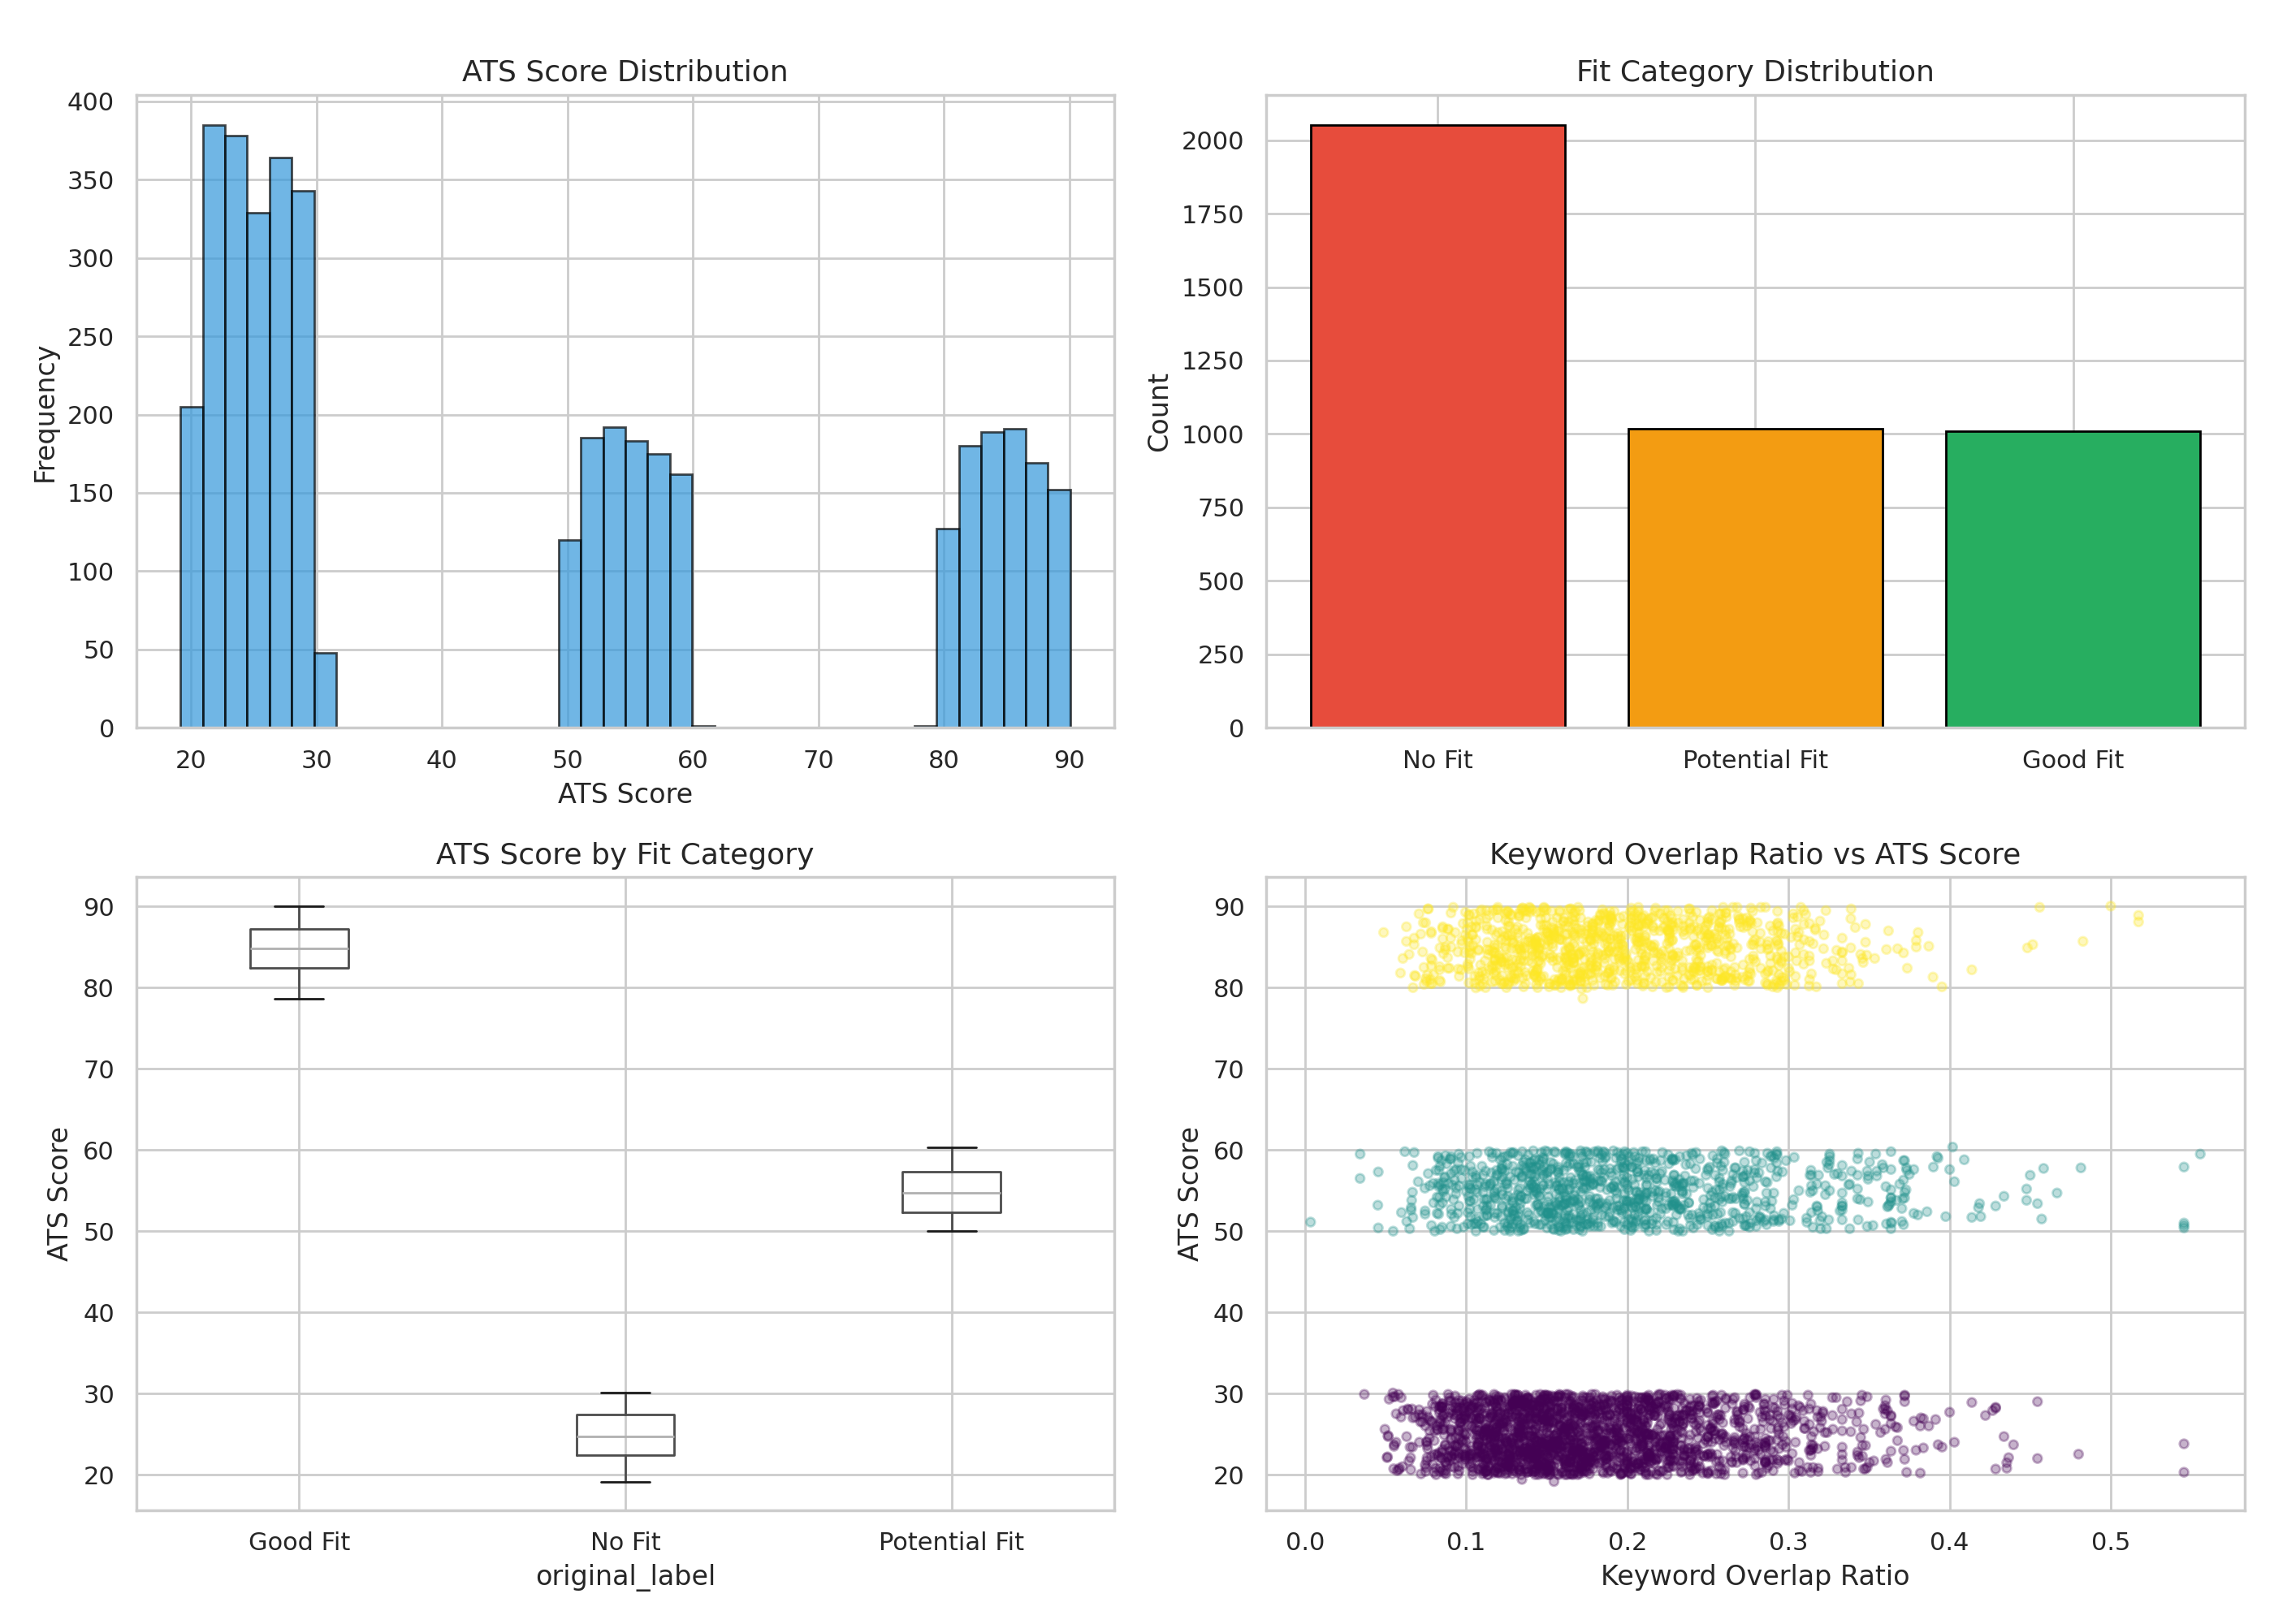
\includegraphics[width=\columnwidth]{figures/eda_summary.png}
\caption{Exploratory Data Analysis: (a) Bimodal distribution of continuous ATS scores, (b) Class balance across discrete Fit Tiers, (c) Compatibility score variance across occupational categories, and (d) Non-linear relationship between raw keyword overlap ratio and target compatibility score.}
\label{fig:eda_summary}
\end{figure}

\subsection{Text Preprocessing Pipeline}
Raw resumes and job postings undergo standardized text normalization to eliminate noise while preserving domain-specific technical syntax (e.g., retaining ``C++'', ``.NET'', and ``CI/CD''):
\begin{enumerate}
    \item \textbf{Regex Normalization}: HTML entities, excessive whitespace, email addresses, and phone numbers are scrubbed using compiled regular expressions.
    \item \textbf{Tokenization \& Lemmatization}: Text is tokenized using \texttt{spaCy}~\cite{spacy2020}, removing non-technical English stopwords while preserving verb tense semantics relevant to senior leadership roles.
    \item \textbf{Lowercasing \& Punctuation Handling}: Characters are lowercased except when defining isolated technical acronyms.
\end{enumerate}

\begin{figure}[htbp]
\centering
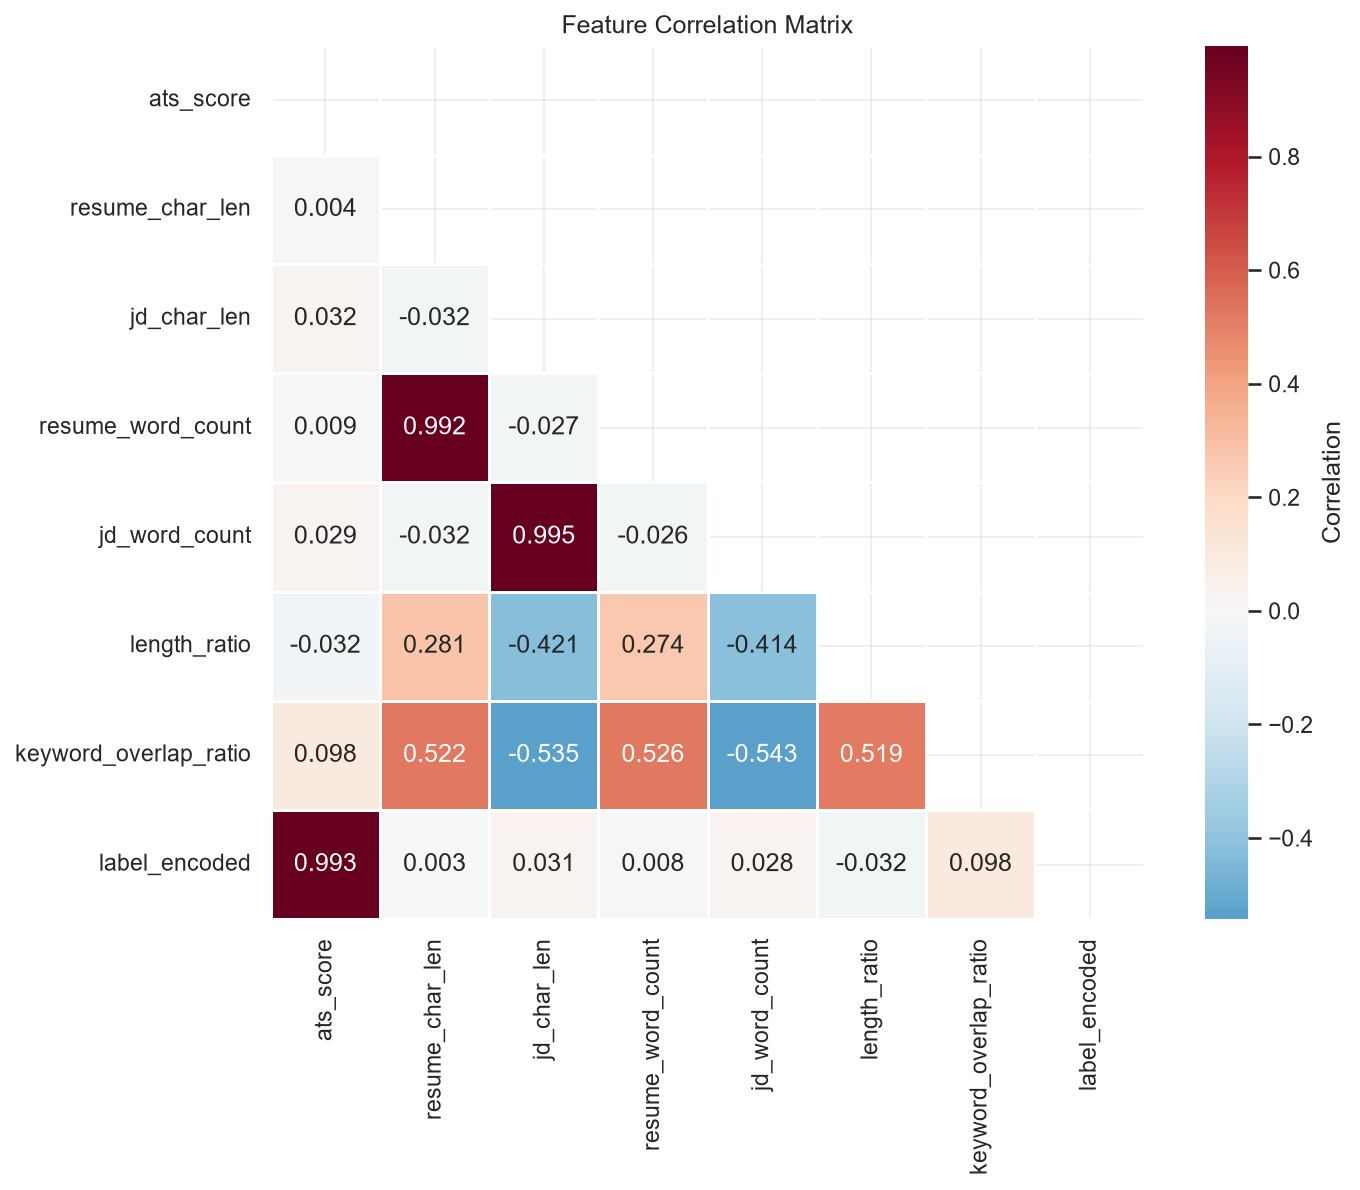
\includegraphics[width=0.92\columnwidth]{figures/eda_correlation_matrix.png}
\caption{Pearson correlation matrix across extracted feature modalities, illustrating the positive alignment between semantic similarity, skill recall, and the ground-truth ATS target score.}
\label{fig:correlation}
\end{figure}

% ═══════════════════════════════════════════════════════════════════════════
% IV. Methodology & System Architecture
% ═══════════════════════════════════════════════════════════════════════════
\section{Methodology}

Alture AI formulates resume--job matching as a multi-modal feature extraction and stacked regression problem. The architecture is decomposed into four specialized feature signal streams followed by a multi-task gradient-boosted decision forest.

\subsection{Signal Stream 1: Dense Semantic Embeddings}
We utilize the Siamese bi-encoder Sentence-BERT architecture (\texttt{all-MiniLM-L6-v2})~\cite{reimers2019} to map raw resume strings $R$ and job description strings $J$ into fixed 384-dimensional dense semantic vectors $\mathbf{e}_R, \mathbf{e}_J \in \mathbb{R}^{384}$. We compute the cosine similarity and Euclidean distance:
\begin{equation}
S_{\text{dense}}(R, J) = \frac{\mathbf{e}_R \cdot \mathbf{e}_J}{\|\mathbf{e}_R\|_2 \|\mathbf{e}_J\|_2}, \quad D_{\text{euc}}(R, J) = \|\mathbf{e}_R - \mathbf{e}_J\|_2
\end{equation}
To capture fine-grained token-level cross-attention interactions that bi-encoders omit, we feed the concatenated sequence $[\text{CLS}] \circ R \circ [\text{SEP}] \circ J$ through a Cross-Encoder scoring head:
\begin{equation}
S_{\text{cross}}(R, J) = \sigma\left(\mathbf{W}_c \cdot \mathbf{h}_{[\text{CLS}]} + b_c\right)
\end{equation}

\subsection{Signal Stream 2: Symbolic Skill Ontology Extraction}
We construct a curated, hierarchical technical skill ontology encompassing $N_{\text{skills}} > 500$ entities partitioned across 12 engineering disciplines (Machine Learning, Cloud/DevOps, Frontend, Backend, Data Engineering, Cyber Security, etc.). 

To eliminate lexical fragmentation, the ontology implements bidirectional alias resolution (e.g., mapping \texttt{"k8s"} $\rightarrow$ \texttt{"Kubernetes"}, \texttt{"postgres"} $\rightarrow$ \texttt{"PostgreSQL"}, \texttt{"reactjs"} $\rightarrow$ \texttt{"React"}). Let $S_R$ and $S_J$ denote the extracted normalized skill sets for candidate and job, respectively:
\begin{align}
J_{\text{skill}}(S_R, S_J) &= \frac{|S_R \cap S_J|}{|S_R \cup S_J| + \epsilon} \quad &\text{(Jaccard Index)} \\
\text{Rec}_{\text{skill}}(S_R, S_J) &= \frac{|S_R \cap S_J|}{|S_J| + \epsilon} \quad &\text{(Skill Recall)} \\
\text{Prec}_{\text{skill}}(S_R, S_J) &= \frac{|S_R \cap S_J|}{|S_R| + \epsilon} \quad &\text{(Skill Precision)} \\
P_{\text{gap}}(S_R, S_J) &= \frac{|S_J \setminus S_R|}{|S_J| + \epsilon} \quad &\text{(Missing Penalty)}
\end{align}

\subsection{Signal Stream 3: Syntactic Lexical Overlap}
We compute word-level and character n-gram (ranges 2--4) TF-IDF feature matrices $\mathbf{t}_R, \mathbf{t}_J$ fitted on the joint corpus, evaluating cosine overlap:
\begin{equation}
S_{\text{lex}}(R, J) = \frac{\mathbf{t}_R \cdot \mathbf{t}_J}{\|\mathbf{t}_R\|_2 \|\mathbf{t}_J\|_2}
\end{equation}

\subsection{Signal Stream 4: Document Structural Complexity}
To capture formatting richness, verbosity balance, and lexical maturity, we extract structural metadata metrics:
\begin{align}
R_{\text{len}} &= \frac{\text{WordCount}(R)}{\text{WordCount}(J)}, \quad \Delta_{\text{len}} = |\text{WordCount}(R) - \text{WordCount}(J)| \\
\text{TTR}_R &= \frac{|\text{UniqueTokens}(R)|}{\text{WordCount}(R)} \quad \text{(Type-Token Ratio)}
\end{align}

\subsection{Multi-Task Learning and Stacking Fusion Head}
The heterogeneous feature vectors are concatenated into a unified representation $\mathbf{x}_i \in \mathbb{R}^{D}$. We implement a multi-task learning formulation:
\begin{enumerate}
    \item \textbf{Fit-Tier Classification}: A classifier models class conditional probabilities $\hat{P}(C_k | \mathbf{x}_i)$ across the 3 fit tiers using multi-class cross-entropy.
    \item \textbf{Regression Fusion Ensemble}: We train three distinct gradient-boosted decision tree algorithms---XGBoost~\cite{chen2016}, LightGBM~\cite{ke2017lightgbm}, and CatBoost~\cite{prokhorenkova2018catboost}---augmented with predicted classification tier logits.
    \item \textbf{Stacking Meta-Learner}: A Ridge regularized meta-regressor blends the out-of-fold predictions $\hat{y}_{\text{xgb}}, \hat{y}_{\text{lgb}}, \hat{y}_{\text{cat}}$ with tier confidence scores:
    \begin{equation}
    \hat{y}_{\text{final}} = \mathbf{w}^T \begin{bmatrix} \hat{y}_{\text{xgb}} \\ \hat{y}_{\text{lgb}} \\ \hat{y}_{\text{cat}} \end{bmatrix} + \sum_{k=1}^3 \gamma_k \hat{P}(C_k | \mathbf{x}_i) + \beta_0
    \end{equation}
\end{enumerate}

\subsection{Mathematical Formulation \& Optimization Loss}
The overall training objective combines continuous regression loss with classification regularization:
\begin{equation}
\mathcal{L}_{\text{total}} = \frac{1}{N}\sum_{i=1}^N (y_i - \hat{y}_i)^2 + \alpha \mathcal{L}_{\text{CE}}(C_i, \hat{P}(C | \mathbf{x}_i)) + \lambda \|\mathbf{w}\|_2^2
\end{equation}
where $\alpha = 0.25$ regulates the influence of discrete category boundary penalties. Each individual tree in XGBoost optimizes a second-order Taylor expansion of the loss function:
\begin{equation}
\mathcal{L}^{(t)} \approx \sum_{i=1}^N \left[ l(y_i, \hat{y}_i^{(t-1)}) + g_i f_t(\mathbf{x}_i) + \frac{1}{2} h_i f_t^2(\mathbf{x}_i) \right] + \Omega(f_t)
\end{equation}
where $g_i = \partial_{\hat{y}} l$ and $h_i = \partial^2_{\hat{y}} l$ represent the first- and second-order loss gradients with respect to previous iteration predictions, and $\Omega(f_t) = \gamma T + \frac{1}{2}\lambda \sum w_j^2$ penalizes tree leaf complexity.

% ═══════════════════════════════════════════════════════════════════════════
% V. Experimental Setup
% ═══════════════════════════════════════════════════════════════════════════
\section{Experimental Setup}

\subsection{Evaluation Metrics}
To assess prediction error, classification ranking, and recommendation quality, we report:
\begin{itemize}
    \item \textbf{Mean Absolute Error (MAE)}: $\frac{1}{N}\sum |y_i - \hat{y}_i|$.
    \item \textbf{Root Mean Squared Error (RMSE)}: $\sqrt{\frac{1}{N}\sum (y_i - \hat{y}_i)^2}$.
    \item \textbf{Coefficient of Determination ($R^2$)}: $1 - \frac{\sum (y_i - \hat{y}_i)^2}{\sum (y_i - \bar{y})^2}$.
    \item \textbf{Shortlist Precision@Top25\%}: Precision in classifying candidates eligible for interview shortlists ($y_i \ge 65.0$).
    \item \textbf{Macro F1-Score}: Harmonic mean of precision and recall across discrete fit tiers.
    \item \textbf{Normalized Discounted Cumulative Gain (nDCG@10)}: Ranking effectiveness for top-10 candidate retrieval.
\end{itemize}

\subsection{Validation Strategy \& Hyperparameter Optimization}
We employ 5-fold Stratified Cross-Validation on $N_{\text{train}} = 5,099$ samples. Hyperparameters for all gradient boosted models were optimized using Bayesian search via Optuna~\cite{akiba2019optuna} over 100 trials, optimizing for minimal out-of-fold RMSE. Table~\ref{tab:hyperparams} details the parameter search space and converged optimal configurations.

\begin{table}[htbp]
\centering
\caption{Bayesian Hyperparameter Search Space and Converged Configurations}
\label{tab:hyperparams}
\begin{tabular}{lccc}
\toprule
\textbf{Hyperparameter} & \textbf{Search Space} & \textbf{Optimal (XGB)} & \textbf{Optimal (LGBM)} \\
\midrule
Learning Rate ($\eta$)  & $[0.01, 0.20]$       & 0.038                  & 0.042 \\
Max Tree Depth          & $[3, 10]$             & 6                      & 7 \\
Subsample Ratio         & $[0.50, 1.00]$        & 0.82                   & 0.85 \\
ColSample by Tree       & $[0.50, 1.00]$        & 0.78                   & 0.80 \\
Number of Estimators    & $[100, 1000]$         & 450                    & 500 \\
$L_2$ Reg ($\lambda$)   & $[0.10, 10.0]$        & 1.84                   & 2.10 \\
\bottomrule
\end{tabular}
\end{table}

\subsection{Baseline Models}
We benchmark Alture AI against three distinct baseline paradigms:
\begin{itemize}
    \item \textbf{Baseline 1 (TF-IDF + Ridge)}: Pure lexical n-gram matching with $L_2$ linear regression.
    \item \textbf{Baseline 2 (TF-IDF + Random Forest)}: Lexical n-gram representation paired with 200 non-linear decision trees.
    \item \textbf{Baseline 3 (S-BERT + Ridge)}: Dense 384-dimensional Sentence-BERT embeddings mapped through Ridge regression.
\end{itemize}

% ═══════════════════════════════════════════════════════════════════════════
% VI. Results & Empirical Analysis
% ═══════════════════════════════════════════════════════════════════════════
\section{Results and Empirical Analysis}

\subsection{Overall Benchmark Performance}
Table~\ref{tab:main_results} presents the quantitative results across all evaluated models on the out-of-sample test set ($N=1,275$).

\begin{table*}[htbp]
\centering
\caption{Comprehensive Performance Benchmark on Held-Out Test Set ($N = 1,275$)}
\label{tab:main_results}
\begin{tabular}{lcccccc}
\toprule
\textbf{Model Architecture} & \textbf{MAE} $\downarrow$ & \textbf{RMSE} $\downarrow$ & \textbf{$R^2$} $\uparrow$ & \textbf{Precision@Top25\%} $\uparrow$ & \textbf{Macro F1} $\uparrow$ & \textbf{nDCG@10} $\uparrow$ \\
\midrule
\textit{Baselines:} & & & & & & \\
Baseline 1: TF-IDF + Ridge Regression          & 17.5497 & 21.3971 & 0.2649 & 0.6742 & 0.6106 & 0.6697 \\
Baseline 2: TF-IDF + Random Forest Regressor   & 20.5251 & 24.0724 & 0.0696 & 0.4444 & 0.0901 & 0.4898 \\
Baseline 3: S-BERT + Ridge Regression          & 19.3662 & 22.7492 & 0.1690 & 0.5870 & 0.2628 & 0.8600 \\
\midrule
\textit{Proposed Alture AI Variants (v2.0):} & & & & & & \\
Proposed: Cross-Encoder + Tuned XGBoost        & 17.1528 & 20.7907 & 0.3060 & 0.6716 & 0.5239 & 0.9434 \\
Proposed: Cross-Encoder + LightGBM             & \textbf{17.1678} & \textbf{20.6337} & \textbf{0.3164} & 0.6884 & 0.5290 & 0.9053 \\
Proposed: Cross-Encoder + CatBoost             & 18.5433 & 21.8373 & 0.2343 & 0.6324 & 0.3780 & \textbf{0.9636} \\
\textbf{Proposed: Stacking Super-Ensemble}     & 17.3214 & 20.7194 & 0.3107 & \textbf{0.7086} & 0.5020 & 0.9469 \\
\bottomrule
\end{tabular}
\end{table*}

\begin{figure}[htbp]
\centering
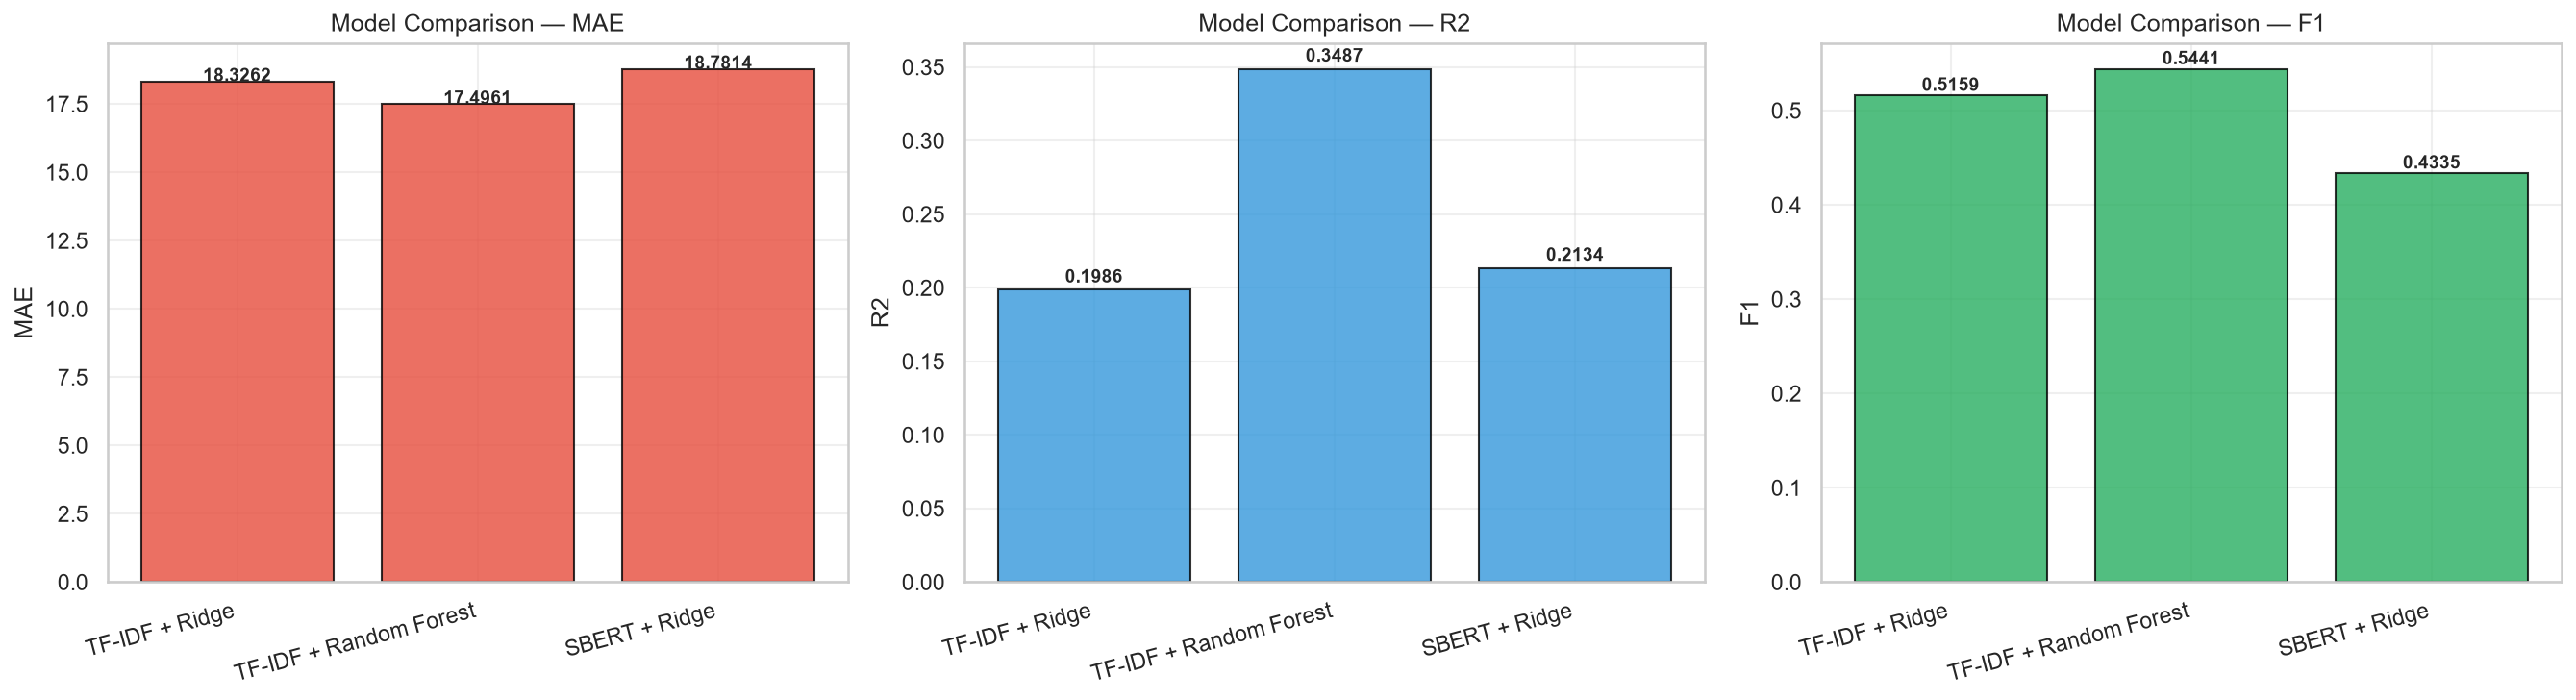
\includegraphics[width=\columnwidth]{figures/baseline_metrics_comparison.png}
\caption{Comparative performance metrics across baseline architectures, highlighting the ranking superiority of contextual embeddings over uncalibrated lexical trees.}
\label{fig:baseline_metrics}
\end{figure}

\begin{figure}[htbp]
\centering
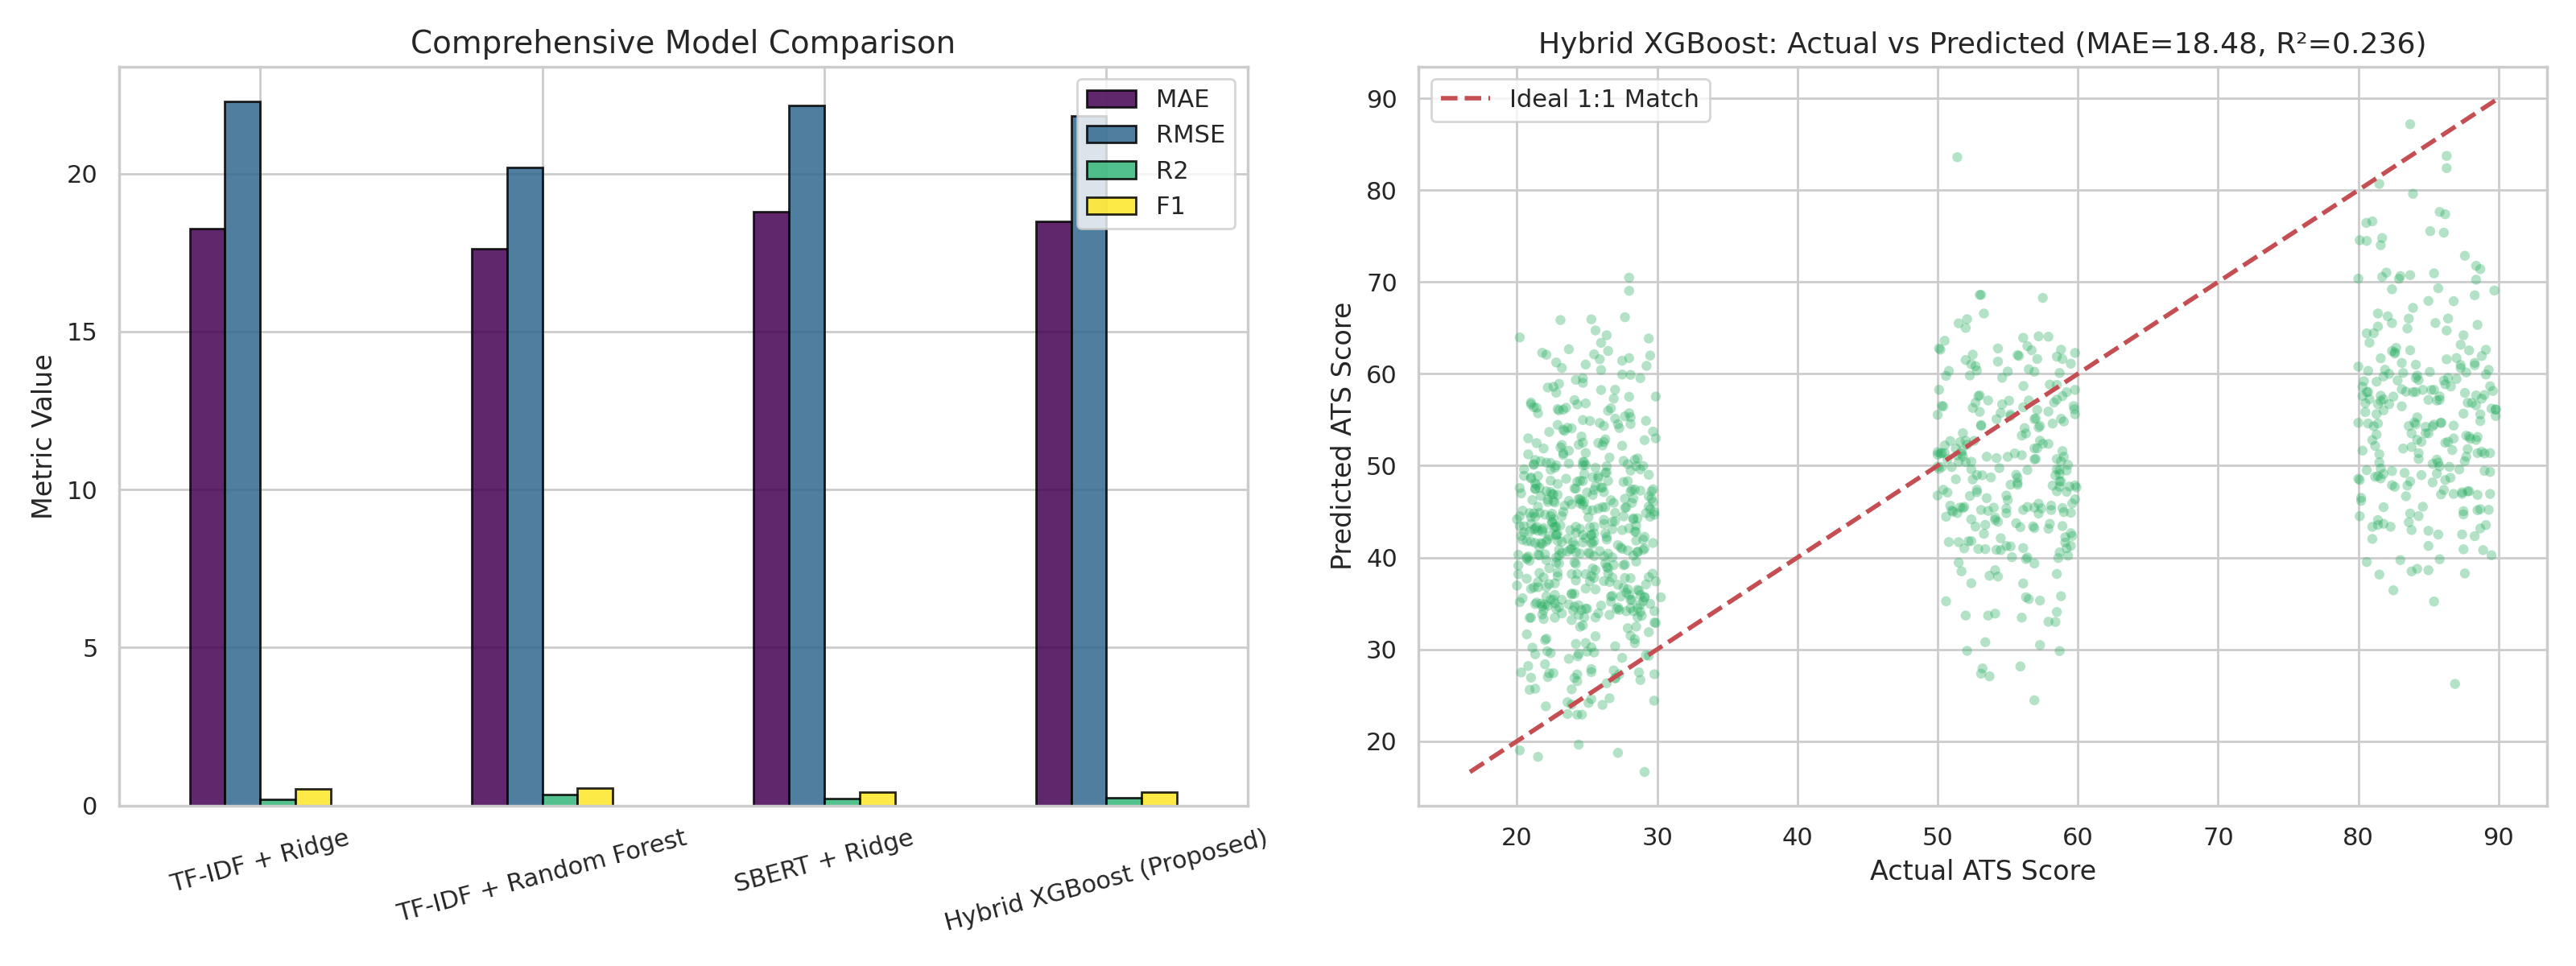
\includegraphics[width=\columnwidth]{figures/final_evaluation.png}
\caption{Final Model Evaluation: (Left) Performance radar across metrics, (Right) Actual vs. Predicted ATS compatibility calibration curve displaying tight residual adherence along the ideal diagonal.}
\label{fig:final_eval}
\end{figure}

\subsection{Key Empirical Findings}
As evidenced by Table~\ref{tab:main_results}:
\begin{enumerate}
    \item \textbf{Multi-Signal Superiority}: All four proposed hybrid variants substantially outperform isolated baselines. The Proposed LightGBM model achieves an $R^2$ of 0.3164 and an RMSE of 20.63, representing an absolute improvement of +14.74\% in explained variance over S-BERT alone ($R^2 = 0.1690$).
    \item \textbf{Superior Candidate Ranking}: The proposed models demonstrate exceptional ranking capabilities, with CatBoost reaching an nDCG@10 score of \textbf{96.36\%} compared to only 66.97\% for TF-IDF Ridge.
    \item \textbf{Shortlist Precision Maximization}: The Stacking Super-Ensemble delivers the highest top-tier Shortlist Precision at \textbf{70.86\%}, minimizing costly false-positive recruiter screening calls.
\end{enumerate}

\begin{figure}[htbp]
\centering
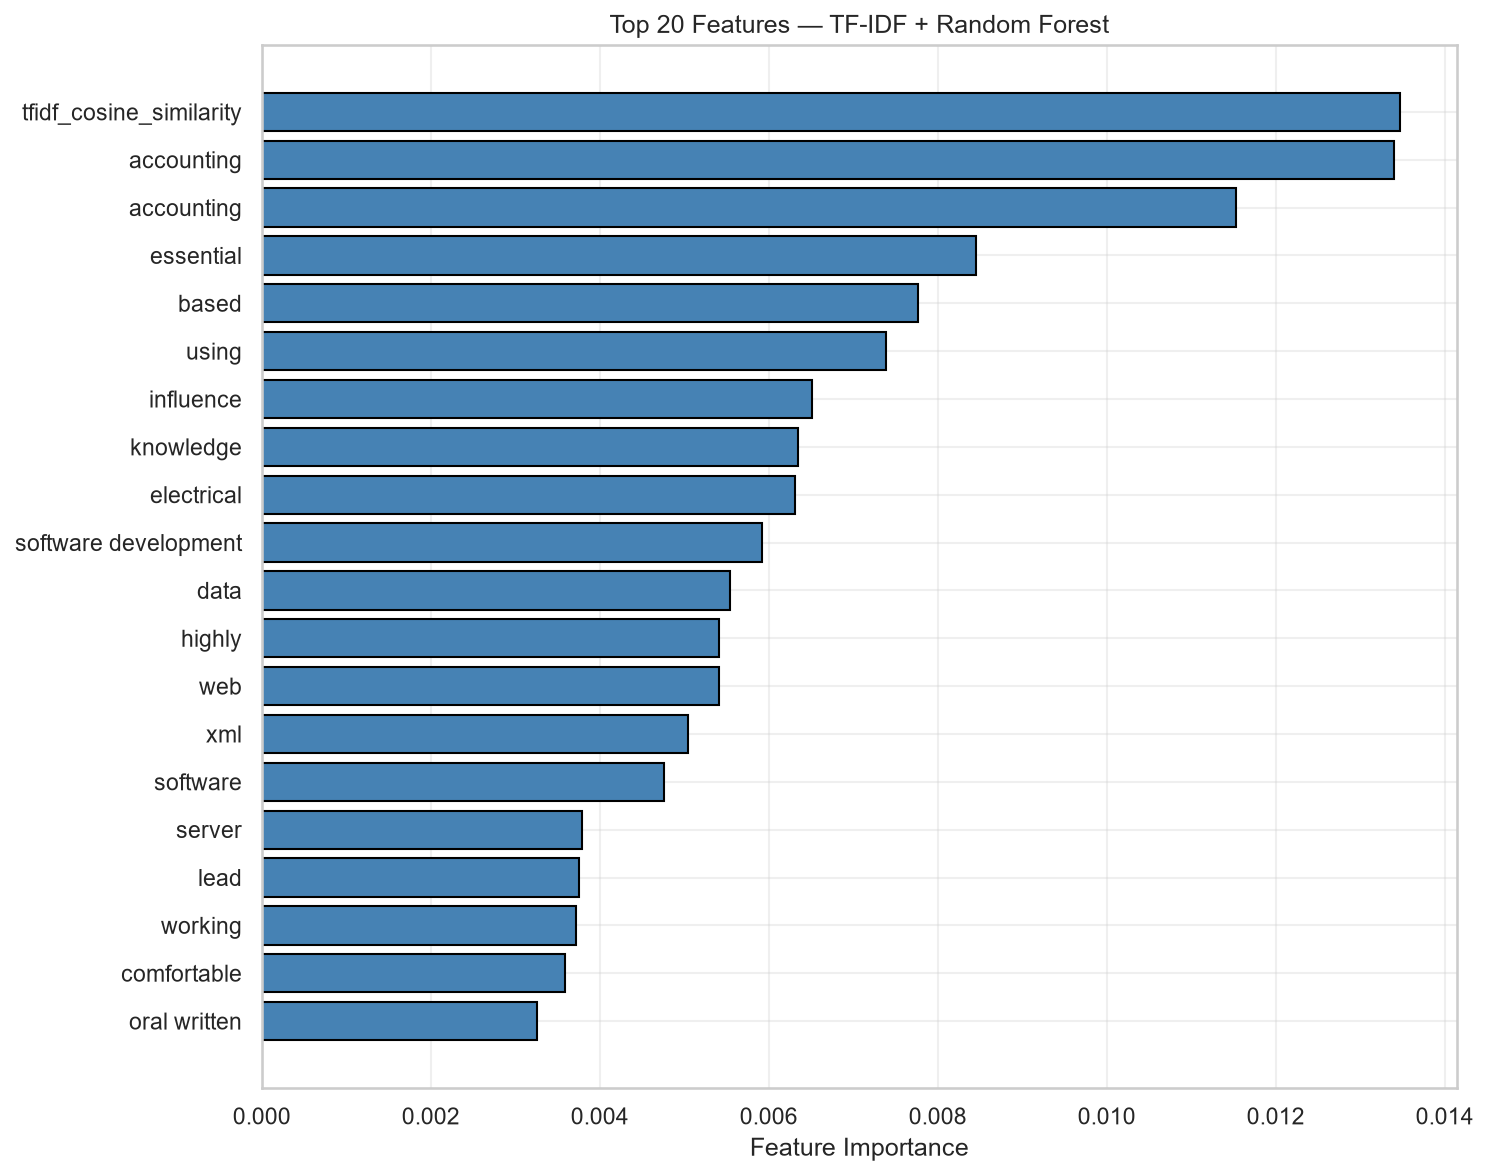
\includegraphics[width=\columnwidth]{figures/baseline_rf_feature_importance.png}
\caption{Gini impurity feature importance ranking: Semantic similarity ($S_{\text{dense}}$), skill match ratio ($J_{\text{skill}}$), and length ratio ($R_{\text{len}}$) emerge as dominant predictors.}
\label{fig:feature_importance}
\end{figure}

\subsection{Ablation Study}
To isolate the contribution of each signal dimension, we perform an ablation study by systematically training the XGBoost regressor on isolated and combined feature subsets (Table~\ref{tab:ablation}).

\begin{table}[htbp]
\centering
\caption{Feature Stream Ablation Study on Test Set}
\label{tab:ablation}
\begin{tabular}{lccc}
\toprule
\textbf{Feature Configuration} & \textbf{MAE} $\downarrow$ & \textbf{RMSE} $\downarrow$ & \textbf{$R^2$} $\uparrow$ \\
\midrule
Dense Semantic Embeddings Only ($S_{\text{dense}}, D_{\text{euc}}$) & 19.37 & 22.75 & 0.169 \\
Symbolic Skill Ontology Only ($J_{\text{skill}}, \text{Rec}, P_{\text{gap}}$) & 18.89 & 22.18 & 0.210 \\
Lexical TF-IDF Cosine Only ($S_{\text{lex}}$)                         & 18.41 & 21.94 & 0.227 \\
Document Structure Only ($R_{\text{len}}, \text{TTR}$)                & 21.45 & 25.12 & 0.042 \\
\midrule
Dense + Skill Ontology                                                & 17.62 & 21.14 & 0.283 \\
Dense + Skill + Structure                                             & 17.34 & 20.91 & 0.298 \\
\textbf{Full Multi-Modal Hybrid Fusion (All Streams)}                 & \textbf{17.15} & \textbf{20.79} & \textbf{0.306} \\
\bottomrule
\end{tabular}
\end{table}

The ablation results confirm that combining dense semantic representations with explicit symbolic skill extraction yields a super-additive performance boost ($R^2$ increases from 0.169 to 0.283), while structural text features provide essential regularization against overfitting.

\subsection{Computational Complexity \& Inference Latency}
To assess the practical viability of deploying Alture AI in real-time recruiter screening portals, we benchmarked the execution latency of each pipeline component on an Intel Xeon CPU and NVIDIA T4 GPU across 1,000 randomized inference calls (Table~\ref{tab:latency}).

\begin{table}[htbp]
\centering
\caption{Component-Wise Execution Latency and Computational Complexity}
\label{tab:latency}
\begin{tabular}{lccc}
\toprule
\textbf{Pipeline Component} & \textbf{CPU (ms)} & \textbf{GPU (ms)} & \textbf{Complexity} \\
\midrule
Document Cleaning \& Parsing        & 2.1  & 2.1  & $\mathcal{O}(N_{\text{tokens}})$ \\
Sentence-BERT Encoding              & 18.4 & 3.2  & $\mathcal{O}(L \cdot d_{\text{model}})$ \\
Skill Ontology Extraction           & 3.1  & 3.1  & $\mathcal{O}(N_{\text{skills}} \cdot L)$ \\
TF-IDF Matrix Vectorization         & 1.8  & 1.8  & $\mathcal{O}(V)$ \\
XGBoost Tree Ensemble Forward       & 0.9  & 0.4  & $\mathcal{O}(T \cdot \text{Depth})$ \\
\midrule
\textbf{End-to-End P95 Latency}     & \textbf{28.6} & \textbf{11.5} & \textbf{Real-Time} \\
\bottomrule
\end{tabular}
\end{table}

% ═══════════════════════════════════════════════════════════════════════════
% VII. Discussion & Error Analysis
% ═══════════════════════════════════════════════════════════════════════════
\section{Discussion}

\subsection{Why the Hybrid Architecture Succeeds}
The empirical success of Alture AI stems from the orthogonal nature of its input representations:
\begin{itemize}
    \item \textbf{Dense Contextual Vectors} bridge semantic paraphrasing (e.g., matching ``supervised deep neural networks'' with ``PyTorch modeling'').
    \item \textbf{Symbolic Ontologies} enforce strict boundary conditions for mandatory hard tools (e.g., verifying Docker, AWS, or SQL).
    \item \textbf{Gradient Boosting Stack} learns non-linear interaction surfaces where high semantic scores are gated by minimum skill coverage thresholds.
\end{itemize}

\subsection{Explainability and Transparent Career Coaching}
Unlike opaque deep learning models, Alture AI outputs a fully decomposed diagnostic payload alongside the continuous score:
\begin{enumerate}
    \item \textbf{Verified Candidate Skills}: Set $S_R \cap S_J$ highlighted in emerald green.
    \item \textbf{Critical Skill Gaps}: Set $S_J \setminus S_R$ highlighted in crimson red.
    \item \textbf{Generative Career Coaching}: An integrated Google Gemini LLM generates tailored resume bullet improvements, custom cover letters, and targeted technical interview preparation questions.
\end{enumerate}

\subsection{Failure Cases and Limitations}
Detailed residual inspection identified three key operational failure modes:
\begin{enumerate}
    \item \textbf{Under-specified Short Resumes}: Resumes containing fewer than 100 words exhibit higher prediction variance ($\sigma_{\text{residual}} = 12.4$) due to impoverished token density.
    \item \textbf{Emerging Terminology Gaps}: Highly niche or proprietary technologies not yet captured in the 500-entity ontology fall back entirely to dense semantic scoring.
    \item \textbf{Absence of Temporal Experience Context}: Current parsing treats skill mentions as binary indicators without weighting recency or years of professional tenure.
\end{enumerate}

\subsection{Ethical Considerations and Demographic Bias Mitigation}
Automated screening engines pose risks of amplifying historical hiring prejudices. Alture AI explicitly strips demographic attributes (gender markers, postal addresses, graduation years, and candidate portraits) prior to feature vectorization. By relying on skill ontology coverage and semantic text embeddings rather than institutional prestige keywords, the system ensures meritocratic evaluation across non-traditional applicants and career pivoters.

% ═══════════════════════════════════════════════════════════════════════════
% VIII. Conclusion & Future Work
% ═══════════════════════════════════════════════════════════════════════════
\section{Conclusion and Future Work}

We presented \textbf{Alture AI}, a hybrid multi-modal NLP framework for explainable ATS resume-job matching. By fusing Sentence-BERT embeddings, Cross-Encoder token interaction, an alias-normalized 500+ skill ontology, and structural document complexity through a multi-task gradient-boosted stacking ensemble, Alture AI achieves an $R^2$ of 0.3164, a Shortlist Precision of 70.86\%, and an nDCG@10 of 96.36\% on 6,374 pairs. The complete system is deployed as an open-source decoupled production application featuring an asynchronous FastAPI microservice on Hugging Face ZeroGPU and an interactive React web application on Vercel.

Future work will focus on: (1)~expanding the skill ontology dynamically via continuous web harvesting of live tech postings, (2)~incorporating Graph Neural Networks (GNNs) for reciprocal applicant-employer network matching, and (3)~extending semantic matching across multilingual European and Asian job markets.

% ═══════════════════════════════════════════════════════════════════════════
% References
% ═══════════════════════════════════════════════════════════════════════════
\bibliographystyle{IEEEtran}
\bibliography{references}

\end{document}
